\documentclass[11pt,oneside]{scrartcl}
\usepackage[a4paper,total={6.5in, 9.0in}]{geometry}

\newcommand{\mchname}{Mat\'{u}\v{s} Chochl\'{i}k}
\newcommand{\mchmail}{chochlik@gmail.com}
\newcommand{\doctitle}{Static reflection}
\newcommand{\docsubtitle}{Rationale, design and evolution.}
\newcommand{\docnum}{DxxxxR0}
\newcommand{\docdate}{2016-04-19}

\usepackage[utf8]{inputenc}
\usepackage{url}
\usepackage[colorlinks=false,hidelinks]{hyperref}
\usepackage{parskip}
\usepackage[titletoc]{appendix}
\usepackage{siunitx}
\usepackage{dirtytalk}
\usepackage{color,soul}
\usepackage{enumitem}

\usepackage{listings}
\usepackage{minted}
\lstset{basicstyle=\footnotesize\ttfamily,breaklines=true}

\usepackage{fancyhdr}
\setlength{\headheight}{14pt}
\pagestyle{fancyplain}
\lhead{\fancyplain{}{\textbf{\docnum} -- \doctitle\\\scriptsize{\docsubtitle}}}
\rhead{}
\rfoot{\fancyplain{}{\thepage}}
\cfoot{}

\usepackage[pdftex]{graphicx}
\DeclareGraphicsExtensions{.pdf}
\graphicspath{{images/}}
\usepackage{rotating}

\setcounter{tocdepth}{3} 

\title{\doctitle}
\subtitle{\docsubtitle}

\author{\mchname (\mchmail)}

\newcommand{\concept}[1]{{\em{#1}}}
\newcommand{\meta}[1]{\textbf{\em{Meta-#1}}}

\begin{document}

\begin{tabular}{r l}
Document number: & \docnum\\
Date: & \docdate\\
Project: & Programming Language C++ \\
Audience: & Reflection (SG7) / EWG \\
Reply-to: & \mchname (\href{mailto:\mchmail}{\mchmail}), Axel Naumann (\href{mailto:Axel.Naumann@cern.ch}{Axel.Naumann@cern.ch})\\
\end{tabular}

\begin{center}
\vskip 2em
{\Huge \doctitle}\\
{\Large \docsubtitle}
\vskip 1em
{\em \mchname, Axel Naumann}
\vskip 2em
\end{center}

\paragraph{Abstract}

The aim of this paper is to provide the rationale driving the
design of the static reflection facility proposed in P0194
(and its predecessors N3996, N4111 and N4451),
to enumerate and describe its potential use-cases
and to keep a written record of its evolution. It also answers questions
frequently asked in regard to the proposal.

\tableofcontents

\section{Introduction}

Reflection and reflective programming can be used
for a wide range of tasks such as implementation of serialization-like operations,
remote procedure calls, scripting, automated GUI-generation,
implementation of several software design patterns, etc.
C++ as one of the most prevalent programming languages 
lacks a standardized reflection facility.

In this paper we propose the addition of native support for
compile-time reflection to C++ and a library built
on top of the metadata provided by the compiler.

The basic static metadata provided by compile-time reflection
should be as complete as possible to be applicable in a wide
range of scenarios and allow to implement custom higher-level
static and dynamic reflection libraries and reflection-based
utilities.

The term \emph{reflection} refers to the ability of a computer program
to observe and possibly alter its own structure and/or its behavior.
This includes building new or altering the existing data structures,
doing changes to algorithms or changing the way the program code
is interpreted. Reflective programming is a particular kind
of \emph{metaprogramming}.

The advantage of using reflection is in the fact that everything
is implemented in a single programming language, and the human-written
code can be closely tied with the customizable reflection-based
code which is automatically generated by compiler metaprograms,
based on the metadata provided by reflection.

The solution proposed in this paper is based on the
\href{http://kifri.fri.uniza.sk/~chochlik/mirror-lib/html/}{\em Mirror}
reflection utilities~\cite{mirror-doc-cpp11} and on several years
of user experience with reflection-based metaprogramming.


\section{Motivation and Scope}

\subsection{Usefullness of reflection}

There is a wide range of computer programming tasks that involve
the execution of the same algorithm on a set of types defined by an
application or on instances of these types, accessing member variables,
calling free or member functions in an uniform
manner, converting data between the language's intrinsic representation and
external formats, etc., for the purpose of implementing the following:

\begin{itemize}

\item serialization or storing of persistent data in a
custom binary format or in XML, JSON, XDR, etc.,

\item (re-)construction of class instances
from external data representations (like those listed above),
from the data stored in a relational database, from data entered by
a user through a user interface or queried through a web service API,

\item automatic generation of a relational schema from the application
object model and object-relational mapping (ORM),

\item support for scripting 

\item support remote procedure calls (RPC) / remote method invocation (RMI),

\item inspection and manipulation of existing objects via a (graphic) user interface
or a web service,

\item visualization of objects or data and the relations between objects or
relations in the data,

\item automatic or semi-automatic implementation of certain software design patterns,

\item etc.

\end{itemize}

There are several aproaches to the implementation of such
functionality. The most straightforward and also usually the most
error-prone is manual implementation. Many of the tasks listed above
are inherently repetitive and basically require to process programming
language constructs (types, structures, containers, functions, constructors,
class member variables, enumerated values, etc.)
in a very uniform way that could be easily transformed into a meta-algorithm.

While it is acceptable (even if not very advantageous)
for example, for a design pattern implementation to be made by a human,
writing RPC/RMI-related code is a task much better suited for a computer.

This leads to the second, heavily used approach: preprocessing
and parsing of the program source text by a (usually very specfic) external
program (documentation generation tool, interface definition language compiler
for RPC/RMI, web service interface generator, a rapid application
development environment with a form designer, etc.) resulting in additional
program source code, which is then compiled into the final application binary.

This approach has several problems. First, it requires the external
tools which may not fit well into the build system or may not be portable
between platforms or be free; second, such tools are task-specific
and many of them allow only a limited, if any, customization of the output.

Another way to automate these tasks is to use reflection,
reflective programming, metaprogramming and generic programming as
explained below.

\subsection{Motivational examples}

This section describes some of the many possible uses of reflection
and reflective programming on concrete real-world examples.

\subsubsection{Factory generator}

As already said above, it is possible (at least partially) to automate 
the implementation of several established software design patterns.
This example shows how to implement a variant of the {\em Factory}
pattern.

By factory we mean here a class, which can create
instances of a {\em Product} type, but does not require that
the caller chooses the manner of the construction (in the programming
language) nor supplies the required arguments directly
in the C++ intrinsic data representation.

So instead of direct construction of a Product type,

\begin{lstlisting}
// get the values of arguments from the user
int arg1 = get_from_user<int>("Product arg1");
double arg2 = get_from_user<double>("Product arg2");
std::string arg3 = get_from_user<std::string>("Product arg3");
//
// call a constructor with these arguments
Product* pp = new Product(arg1, arg2, arg3);
// default construct a Product
Product p;
// copy construct a Product
Product cp = p;
\end{lstlisting}

which involves selection of a specific constructor, getting
the values of the required arguments and possibly converting 
them from an external representation and calling the selected
constructor with the arguments, 
factories pick or let the application user pick the Product's most
appropriate constructor, they gather the necessary parameters
in a generic way and use the selected constructor to create
an instance of the Product:

\begin{lstlisting}
// get data necessary for construction in xml
XMLNode xml_node_1 = get_xml_node(...);
XMLNode xml_node_2 = get_xml_node(...);

// make a factory for the product type
Factory<Product, XMLWalker> xml_factory;

// use the factory to create instances of Product
// from the external representation
Product p = xml_factory(xml_node_1);
Product* pp = xml_factory.new_(xml_node_2);
\end{lstlisting}

One of the interesting features of these factories is,
that they separate the caller (who just needs to get an instance
of the specified type) from the actual method of creation.

By using a factory, the constructor to be called can 
be automatically picked depending on the data available only at run-time
and not be chosen by the programmer (at least not directly
as in the code above). Factory can match
the constructor to best fit the data available in the external
representation (XML or JSON fragment, dataset resulting from a
RDBS query, etc.)

Even more interesting is, that such factories can be
implemented semi-automatically with the help of reflection.

Every factory is a composition of two distinct (an nearly orthogonal)
parts:

\begin{itemize}
\item{Product-type-dependent}: includes the enumeration of Product's
constructors, enumeration of their parameters, information about
the context in which a constructor is called, etc. This part is based
on reflection and independent on the representation of the input data.

\item{Data representation-dependent}: includes the scanning of the
available input data, conversion into C++ intrinsic data representation,
and the selection of the best constructor. This part is user-defined
and specifies how the input data is gathered and converted into the
C++ representation.
\end{itemize}

\begin{figure}[!th]
\centering
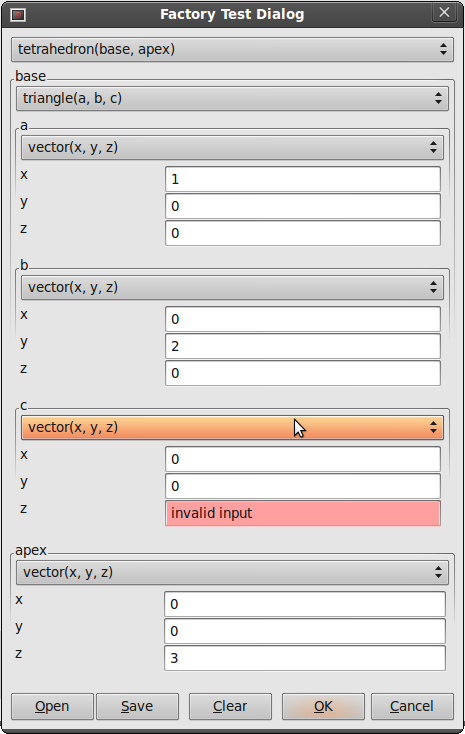
\includegraphics[width=.5\textwidth]{fact_tetrahedron.png}
\caption{Example of a GUI created by a factory generated by
the Mirror's factory generator.}
\label{fig:fact-tetrahedron}
\end{figure}

These two parts are then tied together into the factory class. Based
on the input-data related components, the factory can include a script parser
or XML document tree walker or code dynamically generating a GUI
for the input of the necessary values and the selection of the preferred
constructor. Figure \ref{fig:fact-tetrahedron} shows such a GUI created
by factory automatically generated by the Mirror's {\em factory generator}
utility for a tetrahedron class with the following definition:

\begin{lstlisting}
struct vector
{
        double x,y,z;

        vector(double _x, double _y, double _z)
         : x(_x)
         , y(_y)
         , z(_z)
        { }

        vector(double _w)
         : x(_w)
         , y(_w)
         , z(_w)
        { }

        vector(void)
         : x(0.0)
         , y(0.0)
         , z(0.0)
        { }

        /* other members */
};

struct triangle
{
        vector a, b, c;

        triangle(
                const vector& _a,
                const vector& _b,
                const vector& _c
        ): a(_a)
         , b(_b)
         , c(_c)
        { }

        triangle(void){ }

        /* other members */
};

struct tetrahedron
{
        triangle base;
        vector apex;

        tetrahedron(const triangle& _base, const vector& _apex)
         : base(_base)
         , apex(_apex)
        { }

        tetrahedron(
                const vector& a,
                const vector& b,
                const vector& c,
                const vector& d
        ): base(a, b, c)
         , apex(d)
        { }

        /* other members */
};

\end{lstlisting}


\section{Design Decisions}

\subsection{Desired features} 

The proposed reflection facility is designed with the following
goals in mind:

\begin{itemize}
\item {\em Reusability}: The provided metadata should be reusable
in many situations and for many different purposes, not only
the obvious ones. This is closely related to {\em completeness} (below).

\item {\em Flexibility}: The basic reflection and the libraries
built on top of it should be designed
in a way that they are eventually usable during both compile-time
and run-time and under various paradigms (object-oriented, functional, etc.),
depending on the application needs.

\item {\em  Encapsulation}: The metadata should be accessible
through conceptually well-defined interfaces.

\item {\em  Stratification}: Reflection should be non-intrusive,
and the meta-level should be separated from the base-level language
constructs it reflects. Also, reflection should not be implemented
in a all-or-nothing manner. Things that are not needed, should not generally
be compiled-into the final application.

\item {\em  Ontological correspondence}: The meta-level facilities should
correspond to the ontology of the base-level C++ language constructs
which they reflect. This basically means that all existing language
features should be reflected and new ones should not be invented.
This rule may have some important exceptions like the reflection of
containers.

\item {\em  Completeness}: The proposed reflection facility should
provide as much useful metadata as possible, including various specifiers,
(like constness, storage-class, access, etc.), namespace members,
enumerated types, iteration of namespace members and much more.

\item {\em  Ease of use}: Although reflection-based metaprogramming
allows to implement very complicated things, simple things
should be kept simple.

\item {\em  Cooperation with other librares}: Reflection should be
usable with the existing introspection facilites (like \verb@type_traits@)
already provided by the standard library and with other libraries.
\end{itemize}

\subsection{Layered approach and extensibility}

The purpose of this section is to show that a {\em static} $\to$ {\em dynamic}
and {\em basic} $\to$ {\em complex} approach in designing reflection
can accomodate a wide variety of programming styles and is arguably
the "best" one. It does not propose to add all layers described
below into the standard library.

The Mirror reflection utilities \cite{mirror-doc-cpp11} on which this
proposal is based, implements several distinct components which
are stacked on top of each other. From the low-level metadata, through
a functional-style compile-time interface to a completely dynamic
object-oriented run-time layer (all described in greater detail below).

\subsubsection{Basic metaobjects}
The very basic metadata, which are in Mirror
provided (registered) by the user (or an automated command-line tool) via a set
of preprocessor macros. This approach is both inconvenient and error-prone
in many situations, but also has its advantages.

We propose that a standard compiler would make these basic metadata available
to the programmer through the basic metadata static interfaces. These would
serve as the basis for other (standard and non-standard) higher-level
reflection libraries and utilities.

In the Mirror utilities the basic metadata are not used directly by the
applications.

\subsubsection{Mirror}

A compile-time functional-style reflective programming library,
which is based directly on the basic metadata and is suitable for generic programming,
similar to the standard \verb@type_traits@ library.
It provides a more user-friendly and rich interface than the basic-metaobjects.

Mirror also provides a set of metaprogramming utilities which allow
to write compile-time meta-programs, which can generate efficient
and optimized program code using only those metadata that are required.

The following code shows several (rather simple) examples of usage
and the functional style of the algorithms based on metadata provided by Mirror.

The first example gets all types (registered) in the global scope,
applies some \verb@type_traits@ modifiers like \verb@std::add_pointer@
\verb@std::add_const@ and for each of such modified types calls a functor
that prints the names of the individual types to the standard output:

\begin{lstlisting}
struct name_printer
{
    template <typename MetaNamedObject>
    void operator()(MetaNamedObject mo) const
    {
        std::cout << mo.base_name() << std::endl;
    }
};

int main(void)
{
  using namespace mirror;
  // this function calls the name_printer functor passed
  // as the function argument on each element in the 
  // range that is passed as the template argument
  mp::for_each<
    // this template transforms the elements in the range
    // passed as the first argument by the unary template
    // passed as the second argument
    mp::transform<
      // this template filters out only those metaobjects
      // that satisfy the predicate passed as the second
      // argument from the range of metaobjects passed
      // as the first argument
      mp::only_if<
        // this template "returns" a range of metaobjects
        // reflecting the members of the namespace
        // (or other scope) that is passed as argument
        members<
          // this macro expands into a class
          // conforming to the Mirror's MetaNamespace
          // concept and provides metadata describing
          // the global scope namespace.
          // in the proposed solution for standard C++
          // this would be relaced by a special stdlib
          // function or by an operator.
          MIRRORED_GLOBAL_SCOPE()
        >,
        // this is a lambda function testing if its first
        // argument falls to the MetaType category
        mp::is_a<
          mp::arg<1>,
          meta_type_tag
        >
      >,
      // this is a unary lambda function that modifies the
      // type passed as its argument by the add_pointer
      // and add_const type traits
      apply_modifier<
        mp::arg<1>,
        mp::protect<
          std::add_pointer<
            std::add_const<
              mp::arg<1>
            >
          >
        >
      >
    >
  >(name_printer());
  std::cout << std::endl;
  return 0;
}

\end{lstlisting}


\subsection{Compile-time vs. Run-time reflection}

Run-time, dynamic reflection facilities may seem more readily
usable, but with the increasing popularity of compile-time metaprogramming,
the need for compile-time introspection (already taken care of
by \verb@type_traits@) and reflection also increases.

Also, if compile-time reflection is well supported it is relatively
easy to implement run-time or even dynamically loadable reflection
on top of it. The oposite is not true: One cannot use run-time metaobjects
or the value returned by their member functions as template parameters
or compile-time constants.

From the performance point of view, algorithms based on static
meta-data offer much more possibilities for the compiler to do
optimizations.

Thus, taking shortcuts directly to run-time reflection, without
compile-time support has obvious drawbacks.


\section{Use cases and examples}
\label{use-cases-examples}

Note that some of the examples listed in this section use features which
are not part of the initial reflection specification, but which are planned
as future additions.

\subsection{Portable (type) names}

One of the notorious problems of \verb@std::type_info@ is that the string
returned by its \verb@name@ member function is not standardized and is
not even guaranteed to return any meaningful, unique human-readable string,
at least not without de-mangling, which is platform specific.
Furthermore the returned string is not \verb@constexpr@ and cannot be
reasoned about at compile-time and is applicable only to types.
One other problem with \verb@typeid@ that it is not always aware of \verb@typedef@s.
In some cases we would like to obtain the alias name, instead of the
\say{real} name of a type or a class member or function parameter.

The ability to uniquely map any type used in a program to a human-readable,
portable, compile-time string has several use-cases described in this paper.

The \meta{Named} concept reflects named language constructs
and provides the \verb@get_name@ operation
returning their basic name without any qualifiers or decorations.
This can be with the help of metaprogramming turned into a fully-qualified
name.


\subsection{Logging}

When logging the execution of functions (especialy templated ones) it is sometimes
desirable to also include the names of the parameter types or even the names of the parameters
and other variables.

The best we can do with just the \verb@std::type_info@ is the following:

\begin{minted}[tabsize=4]{cpp}
#if __PLATFORM_ABC__
std::string demangled_type_name(const char*) { /* implementation 1 */ }
#else if __PLATFORM_MNO__
std::string demangled_type_name(const char*) { /* implementation 2 */ }
#else if __PLATFORM_XYZ__
std::string demangled_type_name(const char*) { /* implementation N */ }
#else
std::string demangled_type_name(const char* mangled_name)
{
	// don't know how to demangle this; let's try our luck
	return mangled_name;
}
#endif

template <typename T>
T min(const T& a, const T& b)
{
	log()   << "min<"
	        << demangled_type_name(typeid(T).name())
	        << ">(" << a << ", " << b << ") = ";

	T result = a<b?a:b;

	log()   << result << std::endl;

	return result;
}

\end{minted}

Which may or may not work, depending on the platform.

With the help of reflection as proposed in N4111 we could do:

\begin{minted}[tabsize=4]{cpp}
template <typename T>
T min(const T& a, const T& b)
{
	log()   << "min<"
	        << full_name<mirrored(T)>()
	        << ">(" << a << ", " << b << ") = ";

	T result = a<b?a:b;

	log()   << result << std::endl;

	return result;
}
\end{minted}

The \verb@__PRETTY_FUNCTION__@ macro generated by the compiler could be also
used in this case, but the format of the string which this macro expands into is not customizable
(which may be necessary for logs formatted in XML, JSON, etc.

A more elaborated output containing also the parameter names could be achieved
by using reflection:

\begin{minted}[tabsize=4]{cpp}
template <typename T>
T min(const T& a, const T& b)
{
	log()   << "function: min<"
	        << full_name<mirrored(T)>()
	        << ">"
		<< std::endl
		<< base_name<mirrored(a)>() << ": "
		<< a << std::endl
		<< base_name<mirrored(b)>() << ": "
		<< b << std::endl;

	T result = a<b?a:b;

	log()   << base_name<mirrored(result)>() << ": "
		<< b << std::endl;

	return result;
}
\end{minted}

It is true that the lines:
\begin{minted}[tabsize=4]{cpp}
		<< base_name<mirrored(a)>() << ": "
		<< base_name<mirrored(b)>() << ": "
\end{minted}

could be replaced by preprocessor stringization or just hard coded
strings, like

\begin{minted}[tabsize=4]{cpp}
		<< BOOST_PP_STRINGIZE(a) << ": "
		<< BOOST_PP_STRINGIZE(b) << ": "
\end{minted}

or

\begin{minted}[tabsize=4]{cpp}
		<< "a: "
		<< "b: "
\end{minted}

but the compiler would not force the programmer to change the macro parameter
or the content of the string the if the parameters \verb@a@ and \verb@b@ were renamed
for example to \verb@first@ and \verb@second@. If would enforce the change if
reflection was used.

Furthermore, if the \meta{Function} concept was implemented
and if it was possible to reflect the {\em 'current function'} (i.e. to get a \meta{Function}
from inside of a function body via some invocation of the reflection operator),
then even more would be possible; The function name and even the parameter names could
be obtained from reflection and encapsulated into a function.

\begin{minted}[tabsize=4]{cpp}
template <typename MetaFunction, typename ... P>
void log_function_exec(MetaFunction, const std::tuple<P&...>& params)
{
	log()   << "function: "
		<< base_name<MetaFunction>()
		<< std::endl;

	// obtain the MetaParameter(s) from the MetaFunction
	// and print them pairwise with the values from params.
	for_each<parameters<MetaFunction>>(
		[&params](auto meta_param)
		{
			typedef decltype(meta_param) MP;
			log()  << base_name<MP>() << ": "
			       << std::get<position<MP>::value>(params)
			       << std::endl;
		}
	);
}

template <typename T>
T min(T a, T b)
{
	log_function_exec(mirrored(this::function), std::tie(a, b));
	/* ... */
}

template <typename T>
T max(T a, T b)
{
	log_function_exec(mirrored(this::function), std::tie(a, b));
	/* ... */
}

template <typename T>
T avg(T a, T b)
{
	log_function_exec(mirrored(this::function), std::tie(a, b));
	/* ... */
}
\end{minted}

This example used the following features:

\begin{itemize}
\item{function reflection,}
\item{function parameter reflection,}
\item{context-dependent reflection\footnote{See appendix~\ref{appendix-context-dependent-reflection}.}},
\item{use of metaobject sequences,}
\item{use of the reflection operator,}
\item{base names and the \meta{Named} concept.}
\end{itemize}

\subsection{Generation of common functions}

This use case was part of the \say{targeted use cases} in the committee's
call for compile-time reflection proposals~\cite{ISOCPP-N3814}: 

{\em There are many functions that generally consist of boilerplate code,
performing some action for each member of a class. Such functions include
equality operators, comparison operators, serialization functions,
hash functions and swap functions.
}

In other words for arbitrary structured type, for example:

\begin{minted}[tabsize=4]{cpp}
struct S
{
	int i;
	long l;
	float f;
};
\end{minted}

we want to create equality or non-equality comparison function like:

\begin{minted}[tabsize=4]{cpp}
bool S_equal(const S& a, const S& b)
{
	bool result = true;
	result &= a.i == b.i;
	result &= a.l == b.l;
	result &= a.f == b.f;
	return result;
}

bool S_not_equal(const S& a, const S& b)
{
	bool result = false;
	result |= a.i != b.i;
	result |= a.l != b.l;
	result |= a.f != b.f;
	return result;
}
\end{minted}

or a hash function:

\begin{minted}[tabsize=4]{cpp}
std::size_t S_hash(const S& a)
{
	std::size_t result = 0u;
	result ^= std::hash<int>()(a.i);
	result ^= std::hash<long>()(a.l);
	result ^= std::hash<float>()(a.f);
	return result;
}
\end{minted}

This is one of the many use cases where the \verb@for_each@ function
described in section \ref{fac-for-each} comes in handy. The above could be
implemented along the lines of:

\begin{minted}[tabsize=4]{cpp}
template <typename T>
struct compare_data_members
{
	const T& a;
	const T& b;
	bool& result;

	template <typename MetaDataMember>
	void operator()(identity<MetaDataMember>) const
	{
		auto mem_ptr = meta::get_pointer_v<MetaDataMember>;
		result &= a.*mem_ptr == b.*mem_ptr;
	}
};

template <typename T>
bool generic_equal(const T& a, const T& b)
{
	using metaT = reflexpr(T);
	bool result = true;

	meta::for_each<meta::get_all_data_members_t<metaT>>(
		compare_data_members<T>{a, b, result}
	);

	return result;
}
\end{minted}

If the reversible reflection feature described in section \ref{fut-reverse-reflection}
was implemented then the helper could take advantage of it:

\begin{minted}[tabsize=4]{cpp}
template <typename T>
struct compare_data_members
{
	const T& a;
	const T& b;
	bool& result;

	template <typename MetaDataMem>
	void operator()(identity<MetaDataMem>) const
	{
		result &= a.reflexpr(MetaDataMem) == b.reflexpr(MetaDataMem);
	}
};
\end{minted}

The helper could also be implemented by using a lambda function:

\begin{minted}[tabsize=4]{cpp}

template <typename T>
std::size_t generic_hash(const T& a)
{
	std::size_t result = 0u;

	meta::for_each<meta::get_all_data_members_t<reflexpr(T)>>(
		[&result,&a](auto meta_dm)
		{
			using MetaDataMem = decltype(meta_dm)::type;
			using MetaT = meta::get_type_t<MetaDataMem>;

			using T = meta::get_original_type_t<MetaT>;
			// or T = reflexpr(metaT);

			auto mem_ptr = meta::get_pointer_v<MetaDataMem>;

			result ^= std::hash<T>(a.*mem_ptr);
			// or  ^= std::hash<T>(a.reflexpr(MetaDataMem));
		}
	);

	return result;
}
\end{minted}


\subsection{Enumerator to string and vice versa}
\label{use-case-enum-to-string}

This is another use case from the \say{targeted use cases} in the committee's
call for compile-time reflection proposals~\cite{ISOCPP-N3814}. 

The goal is to automate the implementation of functions which for a given
enumeration value, return the name of the enumeration value:

\begin{minted}[tabsize=4]{cpp}
enum class E
{
	a, b, c, d, e, f
};

string E_to_string(E value)
{
	switch(value)
	{
		case E::a: return "a";
		case E::b: return "b";
		case E::c: return "c";
		case E::d: return "d";
		case E::e: return "e";
		case E::f: return "f";
	}
	return {};
}
\end{minted}

or the other way around:

\begin{minted}[tabsize=4]{cpp}
E string_to_E(const string& name)
{
	if(name == "a") return E::a;
	if(name == "b") return E::b;
	if(name == "c") return E::c;
	if(name == "d") return E::d;
	if(name == "e") return E::e;
	if(name == "f") return E::f;

	// or throw here
	return {};
}
\end{minted}

The Mirror reflection library shows a possible implementation of the
\verb@enum_to_string@,

\begin{minted}[tabsize=4]{cpp}
template <typename Enum>
class enum_to_string
{
private:
	template <typename ... MEC>
	struct _hlpr
	{
		static void _eat(bool ...) { }

		static std::map<Enum, std::string> _make_map(void)
		{
			using namespace std;

			map<Enum, string> res;
			_eat(res.emplace(
				meta::get_constant_v<MEC>,
				string(meta::get_base_name<MEC>())
			).second...);
			return res;
		}
	};
public:
	const std::string& operator()(Enum e) const
	{
		using namespace std;

		using ME = reflexpr(Enum);
		using hlpr = meta::unpack_sequence_t<
			meta::get_enumerators_m<ME>,
			_hlpr
		>;
		static auto m = hlpr::_make_map();
		return m[e];
	}
};
\end{minted}

and the \verb@string_to_enum@ utility:

\begin{minted}[tabsize=4]{cpp}
template <typename Enum>
class string_to_enum
{
private:
	template <typename ... MEC>
	struct _hlpr
	{
		static void _eat(bool ...) { }

		static std::map<std::string, Enum> _make_map(void)
		{
			using namespace std;

			map<string, Enum> res;
			_eat(res.emplace(
				string(meta::get_base_name<MEC>()),
				meta::get_constant_v<MEC>
			).second...);
			return res;
		}
	};
public:
	Enum operator()(const std::string& s) const
	{
		using namespace std;

		using ME = reflexpr(Enum);
		using hlpr = meta::unpack_sequence_t<
			meta::get_enumerators_m<ME>,
			_hlpr
		>;
		static auto m = hlpr::_make_map();
		auto p = m.find(s);
		if(p == m.end()) {
			throw runtime_error("Invalid enumerator name");
		}
		return p->second;
	}
};
\end{minted}


\subsection{Simple serialization}

We need to serialize the instances of selected classes into a structured external format
like XML, JSON, XDR or even into a format like Graphviz dot for the purpose of creating
a visualization of a static class or dynamic object hierarchy or graph.

Reflection makes this task trivial\footnote{
Admittedly this is not the most clever XML schema ever devised, but let's stick to the basics.}:

\begin{minted}[tabsize=4]{cpp}

template <typename T>
void to_xml(const T& instance, std::true_type atomic)
{
	typedef mirrored(T) MetaType;
	std::cout << "<" << base_name<MetaType>() << ">";
	std::cout << instance;
	std::cout << "</" << base_name<MetaType>() << ">";
}

template <typename T>
void to_xml(const T& instance)
{
	to_xml(instance, std::is_fundamental<T>());
}

template <typename T>
void to_xml(const T& instance, std::false_type atomic)
{
	typedef mirrored(T) MetaType;
	std::cout << "<" << base_name<MetaType>() << ">";

	for_each<base_classes<MetaType>>(
		[](auto meta_inheritance)
		{
			typedef decltype(meta_inhertance) MetaInh;
			typedef original_type<base_class<MetaInh>>::type BT;

			to_xml(const BT&(instance));
		}
	);

	for_each<members<MetaType>>(
		[](auto meta_cls_mem)
		{
			typedef decltype(meta_cls_mem) MetaClsMem;
			typedef original_type<type<MetaClsMem>>::type MT;

			if(std::is_base_of<
				meta_variable_tag,
				metaobject_category<MetaClsMem>
			>())
			{
				auto mvp = pointer<MetaClsMem>::get();
				std::cout << "<" << base_name<MetaClsMem> << ">";
				to_xml(instance.*mvp);
				std::cout << "</" << base_name<MetaClsMem> << ">";
			}
		}
	);

	std::cout << "</" << base_name<MetaType>() << ">";
}

\end{minted}

Where necessary explicit specializations can override the generic implementation:

\begin{minted}[tabsize=4]{cpp}

template <typename Bool>
void to_xml(const std::string& instance, Bool)
{
	std::cout << "<string>";
	std::cout << instance;
	std::cout << "</string>";
}

\end{minted}

This use-case shows the following:

\begin{itemize}
\item{class member reflection,}
\item{inheritance reflection,}
\item{class member variable reflection,}
\item{use of metaobject sequences,}
\item{use of the interface of various metaobjects,}
\item{use of the reflection operator,}
\item{metaobject categorization,}
\item{base names and the \meta{Named} concept.}
\end{itemize}


\subsection{Cross-cutting aspects}

We need to execute the same action (or a set of actions) at the entry of or at the exit from the body of
a function (from a set of multiple functions meeting some conditions) each time it is called.

The action may be related to logging, debugging, profiling, but also access control, etc.
The condition which selects the functions for which the action is invoked might be something like:
\begin{itemize}
\item each member function of a particular class,
\item each function defined in some namespace,
\item each function returning values of a particular type or having a particular set of parameters,
\item each function whose name matches a search expression,
\item each function declared in a particular source file,
\item etc. and various combinations of the above.
\end{itemize}

It may not be possible to tell in advance the relations between the aspects and the individual functions
or these relations may vary for different builds or build configurations.
Furthermore we want to be able to quickly change the assignment of actions to functions in one
place instead of going through the whole project source which may consists of dozens or even hundreds of files.

We want for example temporarily enable logging of the entry and exit of each member function of class \verb@foo@,
or we need to count the number of invocations of functions defined in the \verb@bar@ namespace with
names not starting with an underscore, or we want to throw the \verb@not_logged_in@ exception at the entry
of each member function of class \verb@secure@ if the global \verb@user_logged_in@ function returns \verb@false@.

Without reflection something like this could be implemented in the following way:

\begin{minted}[tabsize=4]{cpp}

class logging_aspect
{
public:
	template <typename ... P>
	logging_aspect(const char* func_name, P&&...)
	{
		// write to clog
	}
};

class profiling_aspect
{
	/* ... */
};

class authorization_aspect
{
public:
	template <typename ... P>
	authorization_aspect(const char* func_name, P&&...)
	{
		if(contains(func_name, "secure"))
		{
			if(!::is_user_logged_in())
			{
				throw not_authorized(func_name);
			}
		}
	}
};

template <typename RV, typename ... P>
class func_aspects
 : logging_aspect
 , profiling_aspect
 , authorization_aspect
/* ... etc. ... */
{
public:
	func_aspects(
		const char* name,
		const char* file,
		unsigned line,
		P&&... args
	): logging_aspect(name, file, line, args...)
	 , profiling_aspect(name, file, line, args...)
	 , authorization_aspect(name, file, line, argc...)
	/* ... etc. ... */
	{ }
};

template <typename RV, typename ... P>
func_aspects<RV, P...>
make_func_aspects(
	const char* name,
	const char* file,
	unsigned line,
	P&&...args
);


void func1(int a, int b)
{
	auto _fa = make_func_aspects<void>(
		__func__,
		__FILE__,
		__LINE__,
		a, b
	);
	/* function body */
}

double func2(double a, float b, long c)
{
	auto _fa = make_func_aspects<double>(
		__func__,
		__FILE__,
		__LINE__,
		a, b, c
	);
	/* function body */
}

namespace foo {

long func3(int x)
{
	auto _fa = make_func_aspects<long>(
		__func__,
		__FILE__,
		__LINE__,
		x
	);
	/* function body */
}

} // namespace foo
\end{minted}

Obviously this is very repetitive and it can get quite tedious and error-prone
to supply all this information to the aspects in each function manually.
Also if the signature or the name of the function changes the construction
of the \verb@func_aspects@ instance must be updated accordingly.
With the help of reflection things can be simplified considerably:

\begin{minted}[tabsize=4]{cpp}

template <typename MetaFunction, typename Enabled>
class logging_aspect_impl;

template <typename MetaFunction>
class logging_aspect_impl<MetaFunction, false_type>
{ };

template <typename MetaFunction>
class logging_aspect_impl<MetaFunction, true_type>
{
public:
	logging_aspect_impl(void)
	{
		clog
			<< base_name<MetaFunction>()
			<< "("
			/* ... */
			<< ")"
			<< endl;
	}
};

template <typename MetaFunction>
struct logging_enabled
 : integral_constant<
	bool,
	is_base_of<mirrored(std), scope<MetaFunction>>() &&
	is_same<std::string, original_type<result<MetaFunction>>::type> &&
	/* ... etc. ... */
>
{ };

template <typename MetaFunction>
using logging_aspect =
	logging_aspect_impl<
		MetaFunction,
		typename logging_enabled<MetaFunction>::type
	>;

template <typename MetaFunction, typename Enabled>
class authorization_aspect_impl;

template <typename MetaFunction>
class authiorization_aspect_impl<MetaFunction, false_type>
{ };

template <typename MetaFunction>
class authorization_aspect_impl<MetaFunction, true_type>
{
public:
	authorization_aspect_impl(void)
	{
		if(!::is_user_logged_in())
		{
			throw not_authorized(
				full_name<MetaFunction>()
			);
		}
	}
};

template <typename MetaFunction>
struct autorization_enabled
 : integral_constant<
	bool,
	is_base_of<mirrored(foo::bar), scope<MetaFunction>>() &&
	constexpr_starts_with(base_name<MetaFunction>(), "secure_") &&
	/* ... etc. ... */
>
{ };

template <typename MetaFunction>
using authorization_aspect =
	authorization_aspect_impl<
		MetaFunction,
		typename authorization_enabled<MetaFunction>::type
	>;

template <typename MetaFunction>
class func_aspects
 : logging_aspect<MetaFunction>
 , profiling_aspect<MetaFunction>
 , authorization_aspect<MetaFunction>
/* ... etc. ... */
{
public:
};

void func1(int a, int b)
{
	func_aspects<mirrored(this::function)> _fa;
	/* function body */
}

double func2(double a, float b, long c)
{
	func_aspects<mirrored(this::function)> _fa;
	/* function body */
}

namespace foo {

long func3(int x)
{
	func_aspects<mirrored(this::function)> _fa;
	/* function body */
}

} // namespace foo

\end{minted}

In this case the same expression is used in all functions
regardless of their name and signature and the aspects get all the information
they require from the metaobject reflecting the function. All the data
obtained from the metaobjects is available at compile-time so various
specializations of the aspect classes can be implemented as required.

This same technique could also be used with instances of classes:

\begin{minted}[tabsize=4]{cpp}

template <typename MetaClass>
class class_aspects
 : logging_aspects<MetaClass>
/* ... etc. ... */
{
public:
	class_aspects(typename original_type<MetaClass>::type* that);
};

class cls1
{
private:
	int member1;
	/* ... other members ... */
	class_aspect<mirrored(this::class)> _ca;
public:
	cls1(void)
	 : member1(...)
	 , _ca(this)
	{ }
};

\end{minted}

Class aspects like these could also be used for logging, monitoring of object instantation,
leak detection, etc.

This use-case shows the following:

\begin{itemize}
\item{current function reflection,}
\item{current class reflection.}
\end{itemize}


\subsection{Implementing the factory pattern}

The purpose of the {\em Factory} pattern is to separate its caller,
who requires a new instance of a {\em Product} type, from the details
of this instance's construction. The caller only supplies the input data
to the factory and collects the new instance. There are several aspects
that need to be considered when designing and implementing a factory.

The input data for the construction of an instance of the {\em Product}
can be stored in an external representation (an XML fragment, a RDBS database dataset,
a JSON document, etc.) or even entered by the user through a GUI oron the
command-line and so on, and would need to be converted into a native C++ representation.
The new instance also might be constructed as a copy of another already existing
\emph{prototype} instance of the same type sitting in an object pool.

The product may be polymorphic and the exact type may not even be
known to the user. It may have one or several constructors, each of which
may require a different set of arguments. It may or may not have
constructors with a specific signature, for example a default constructor.

A default constructor does not make sense for many types and requiring it
just because the type will be used with a factory is problematic\footnote{
or even impossible with third-party code}.
Consider for example what a \say{default} instance of \verb@person@ or \verb@address@ would
look like -- it would not have any meaning at all.
Thus well-designed factories should not depend on the presence of constructors
with specific signatures.

Furthermore it might be desirable, that the constructor used to construct
a particular instance is picked based on the available input data which is known
only at run-time, but not when the factory is designed and implemented.

Let's consider the implementation of a factory for a rather simple \verb@point@ class,
representing a point in 3-dimensional space:

\begin{minted}[tabsize=4]{cpp}
struct point
{
    double _x, _y, _z;

    point(double x, double y, double z): _x(x), _y(y), _z(z) { }

    point(double w): _x(w), _y(w), _z(w) { }

    point(void): _x(0.0), _y(0.0), _z(0.0) { }

    point(const point&) = default;

    // ... other declarations
};
\end{minted}

A naive hand-coded implementation, of a factory constructing
\verb@point@s from some \verb@Data@ type (for example an XML node) might look like this:

\begin{minted}[tabsize=4]{cpp}
class point_factory
{
private:
    unsigned pick_constructor(Data data)
    {
        // somehow examine the data and pick
        // the most suitable constructor of the point class
    }

    double extract(Data data, string param)
    {
        // somehow extract and convert the value
        // of a named parameter from the data
    }
public:
    point create(Data data)
    {
        switch(pick_constructor(data))
        {
            case 0: return point();

            case 1: return point(extract(data, "w"));

            case 2: return point(
                        extract(data, "x"),
                        extract(data, "y"),
                        extract(data, "z")
                    );

            default: throw exception(...);
        }
    }
};
\end{minted}

Now suppose that there is some pool of existing \verb@point@ objects
and let's extend the factory to use this pool and return copies if applicable:

\begin{minted}[tabsize=4]{cpp}

extern pool_of<point>& point_pool;

class point_factory
{
private:
    unsigned pick_constructor(Data data)
    {
        // same as before but also allow the copy
        // constructor to be picked if the data says so
    }

    double extract(Data data, string param);
public:
    point create(Data data)
    {
        switch(pick_constructor(data))
        {
            // same as before, but add a new case
            // returning copies from the pool

            case 3: return point_pool.get(data);

            default: throw exception(...);
        }
    }
};
\end{minted}

When looking at the hand-coded factories above, it is obvious that
implementing and maintaining\footnote{as the constructed types evolve and change}
factories for several dozens of classes in a larger
application is a highly repetitive, tedious and possibly error-prone
process and at least partial automation is desirable.

Factory classes must generally handle several tasks
which fit into two distinct and nearly orthogonal categories:

\begin{itemize}
\item{\emph{Product type-related}}
        \begin{itemize}
        \item{\emph{Constructor description}} -- providing the metadata describing
        the individual constructors, their parameters, etc.
        \item{\emph{Constructor dispatching}} -- calling the selected constructor.
        with the supplied arguments which results in a new instance of the product type.
        \end{itemize}

\item{\emph{Input data representation-related}}
        \begin{itemize}
        \item{\emph{Input data validation}} -- checking if the input data match
        the available constructors.
        \item{\emph{Constructor selection}} -- examining the input data, comparing it
        to the metadata describing product's constructors and determining
        which constructor should be called.
        \item{\emph{Getting the argument values}} -- determining where the argument
        values should come from and getting them:
                \begin{itemize}
                \item{\emph{Conversion from the external representation}} -- this usually applies
                to intrinsic C++ types, but complex types could be converted directly too.
                \item{\emph{Recursive construction by using another factory}} -- this usually
                requires some form of cooperation between the parent and its child factories
                and it means that all the tasks discussed here must be repeated also for
                the recursively constructed parameter(s).
                \item{\emph{Copying an existing instance}} -- for example from an object pool.
                \end{itemize}
        \end{itemize}
\end{itemize}

Parts from each category can be combined with parts from the other to create new
factories which promotes code re-usability. Factories constructing instances of a single
product from various data representations share the product-related components
and factories constructing instances of various product types from a single input data representation
share the input-data-related parts. This approach has several advantages like better
maintainability or the ability to develop the components separately and combine them later
via metaprogramming.

If the input data for a metaprogram generating the factory class, that is
the metadata describing the Product type\footnote{specifically the constructors of Product}
can be obtained by using compile-time reflection then new factory classes can be generated
automatically for nearly arbitrary type provided that the input data type-related parts are
implemented.

\subsection{SQL schema generation}

We need to create an SQL/DDL (data definition language) script for creating a schema
with tables which will be storing the values of all structures in namespace C++ \verb@foo@
having names starting with \verb@persistent_@:

\begin{minted}[tabsize=4]{cpp}

const char* translate_to_sql(const std::string& type_name)
{
	if(type_name == "int")
		return "INTEGER";
	/* .. etc. */
}

template <typename MetaMemVar>
void create_table_column_from(MetaMemVar)
{
	if(!std::is_base_of<
		variable_tag,
		metaobject_category<MetaMemVar>
	>()) return;

	std::cout << base_name<MetaMemVar>() << " ";

	std::cout << translate_to_sql(base_name<type<MetaMemVar>());

	if(starts_with(base_name<MetaMemVar>(), "id_"))
	{
		std::cout << " PRIMARY KEY";
	}
	std::cout << std::endl;
}

template <typename MetaClass>
void create_table_from(MetaClass)
{
	if(!std::is_base_of<
		class_tag,
		metaobject_category<MetaClass>
	>()) return;

	std::cout << "CREATE TABLE "
	          << strip_prefix("persistent_", base_name<MetaClass>())
	          << "(" << std::endl;

	for_each<members<MetaClass>>(create_table_column_from);

	std::cout << ");"
}

template <typename MetaNamespace>
void create_schema_from(MetaNamespace)
{
	std::cout << "CREATE SCHEMA "
	          << base_name<MetaNamespace>()
	          << ";" << std::endl;

	for_each<members<MetaNamespace>>(create_table_from);
}

int main(void)
{
	create_schema_from(reflected(foo));
	return 0;
}

\end{minted}

This example shows the following features from N4111:

\begin{itemize}
\item{namespace reflection,}
\item{namespace member reflection,}
\item{class member reflection,}
\item{use of metaobject sequence,}
\item{metaobject categorization,}
\item{base names and the \meta{Named} concept.}
\end{itemize}

Furthermore reflection could be used to implement actual object-relational mapping,
together with a library like \verb@SOCI@, \verb@ODBC@, \verb@libpq@, etc.

\subsection{Structure data member transformations}
\label{use-case-struct-transf}

We need to create a new structure, which has data members with the same names
as an original structure, but we need to change some of the properties
of the data members (for example their types).

For example we need to transform:

\begin{minted}[tabsize=4]{cpp}

struct foo
{
	bool b;
	char c;
	double d;
	float f;
	std::string s;
};

\end{minted}

into

\begin{minted}[tabsize=4]{cpp}

struct rdbs_table_placeholder_foo
{
	column_placeholder<bool>::type b;
	column_placeholder<char>::type c;
	column_placeholder<double>::type d;
	column_placeholder<float>::type f;
	column_placeholder<std::string>::type s;
};

\end{minted}

By using the proposed \verb@identifier@ operator\footnote{See appendix~\ref{appendix-operator-identifier}.}, class member reflection
and multiple inheritance we can create a new structure that is
nearly equivalent to \verb@rdbs_table_foo@ via metaprogramming:

\begin{minted}[tabsize=4]{cpp}

template <typename MetaVariable>
struct rdbs_table_placeholder_helper
{
	typename column_placeholder<
		typename original_type<type<MetaVariable>>::type
	>::type identifier(base_name<MetaVariable>::value);
};

template <typename ... MetaVariables>
struct rdbs_table_placeholder_helpers
 : rdbs_table_placeholder_helper<MetaVariables>...
{ };

template <typename MetaVariableSeq, typename IdxSeq>
class rdbs_table_impl;

template <typename MetaVariableSeq, std::size_t ... I>
class rdbs_table_impl<MetaFunctionSeq, std::index_sequence<I...>>
 : public rdbs_table_placeholder_helpers<at<MetaFunctionSeq, I>...>
{ };

typedef rdbs_table_impl<
	members<mirrored(foo)>,
	std::make_index_sequence<size<members<mirrored(foo)>>::value>
> rdbs_table_placeholder_foo;

\end{minted}

This examples uses the following features.

\begin{itemize}
\item{class member reflection,}
\item{use of the reflection operator,}
\item{use of the \verb@identifier@ operator or the \verb@named_mem_var@ templates.}
\end{itemize}


%\subsection{Replacing Qt's MOC with standard C++}
\label{use-case-replacing-moc}

Replacing the functionality currently provided by the Qt's meta-object
compiler -- an external tool implementing some basic reflection capabilities
and the signal slot mechanism, with standard C++, is another relatively important
use case to be considered when designing C++ reflection.

TODO


\subsection{Simple examples of usage}
\label{working-examples}

This section shows several simple, but complete examples of usage already working
with the experimental implementation of the initial specification.

\subsubsection{Scope reflection}

\begin{minted}[tabsize=4]{cpp}
#include <reflexpr>
#include <iostream>

namespace foo {

struct bar
{
	typedef int baz;
};

} // namespace foo

typedef long foobar;

int main(void)
{
	using namespace std;

	typedef reflexpr(int) meta_int;
	typedef reflexpr(foo::bar) meta_foo_bar;
	typedef reflexpr(foo::bar::baz) meta_foo_bar_baz;
	typedef reflexpr(foobar) meta_foobar;

	static_assert(meta::has_scope_v<meta_int>, "");
	static_assert(meta::has_scope_v<meta_foo_bar>, "");
	static_assert(meta::has_scope_v<meta_foo_bar_baz>, "");
	static_assert(meta::has_scope_v<meta_foobar>, "");

	typedef meta::get_scope_m<meta_int> meta_int_s;
	typedef meta::get_scope_m<meta_foo_bar> meta_foo_bar_s;
	typedef meta::get_scope_m<meta_foo_bar_baz> meta_foo_bar_baz_s;
	typedef meta::get_scope_m<meta_foobar> meta_foobar_s;

	static_assert(meta::is_scope_v<meta_int_s>, "");
	static_assert(meta::is_scope_v<meta_foo_bar_s>, "");
	static_assert(meta::is_scope_v<meta_foo_bar_baz_s>, "");
	static_assert(meta::is_scope_v<meta_foobar_s>, "");

	static_assert(meta::is_namespace_v<meta_int_s>, "");
	static_assert(meta::is_global_scope_v<meta_int_s>, "");
	static_assert(meta::is_namespace_v<meta_foo_bar_s>, "");
	static_assert(!meta::is_global_scope_v<meta_foo_bar_s>, "");
	static_assert(meta::is_type_v<meta_foo_bar_baz_s>, "");
	static_assert(meta::is_class_v<meta_foo_bar_baz_s>, "");
	static_assert(!meta::is_namespace_v<meta_foo_bar_baz_s>, "");
	static_assert(meta::is_namespace_v<meta_foobar_s>, "");
	static_assert(meta::is_global_scope_v<meta_foobar_s>, "");
	static_assert(!meta::is_class_v<meta_foobar_s>, "");

	cout << meta::get_name_v<meta_foo_bar_baz> << endl;
	cout << meta::get_name_v<meta_foo_bar_baz_s> << endl;
	cout << meta::get_name_v<meta_foo_bar_s> << endl;

	return 0;
}
\end{minted}

Output:

\begin{verbatim}
baz
bar
foo
\end{verbatim}


\subsubsection{Namespace reflection}

\begin{minted}[tabsize=4]{cpp}
#include <reflexpr>
#include <iostream>

namespace foo { namespace bar { } }

namespace foobar = foo::bar;

int main(void)
{
	using namespace std;

	typedef reflexpr(foo) meta_foo;

	static_assert(is_metaobject_v<meta_foo>, "");

	static_assert(!meta::is_global_scope_v<meta_foo>, "");
	static_assert(meta::is_namespace_v<meta_foo>, "");
	static_assert(!meta::is_type_v<meta_foo>, "");
	static_assert(!meta::is_alias_v<meta_foo>, "");

	static_assert(meta::has_name_v<meta_foo>, "");
	static_assert(meta::has_scope_v<meta_foo>, "");
	cout << meta::get_name_v<meta_foo> << endl;

	typedef reflexpr(foo::bar) meta_foo_bar;

	static_assert(is_metaobject_v<meta_foo_bar>, "");

	static_assert(!meta::is_global_scope_v<meta_foo_bar>, "");
	static_assert(meta::is_namespace_v<meta_foo_bar>, "");
	static_assert(!meta::is_type_v<meta_foo_bar>, "");
	static_assert(!meta::is_alias_v<meta_foo_bar>, "");

	static_assert(meta::has_name_v<meta_foo_bar>, "");
	static_assert(meta::has_scope_v<meta_foo_bar>, "");
	cout << meta::get_name_v<meta_foo_bar> << endl;

	typedef reflexpr(foobar) meta_foobar;

	static_assert(is_metaobject_v<meta_foobar>, "");

	static_assert(!meta::is_global_scope_v<meta_foobar>, "");
	static_assert(meta::is_namespace_v<meta_foobar>, "");
	static_assert(!meta::is_type_v<meta_foobar>, "");
	static_assert(meta::is_alias_v<meta_foobar>, "");

	static_assert(meta::has_name_v<meta_foobar>, "");
	static_assert(meta::has_scope_v<meta_foobar>, "");
	cout << meta::get_name_v<meta_foobar> << " a.k.a ";
	cout << meta::get_name_v<meta::get_aliased_t<meta_foobar>> << endl;

	return 0;
}
\end{minted}

Output:

\begin{verbatim}
foo
bar
foobar a.k.a bar
\end{verbatim}


\subsubsection{Type reflection}

\begin{minted}[tabsize=4]{cpp}
#include <reflexpr>
#include <iostream>

int main(void)
{
	using namespace std;

	typedef reflexpr(unsigned) meta_unsigned;

	static_assert(is_metaobject_v<meta_unsigned>, "");
	static_assert(meta::is_type_v<meta_unsigned>, "");
	static_assert(!meta::is_alias_v<meta_unsigned>, "");

	static_assert(is_same_v<
		meta::get_reflected_type_t<meta_unsigned>,
		unsigned
	>, "");

	static_assert(meta::has_name_v<meta_unsigned>, "");
	cout << meta::get_name_v<meta_unsigned> << endl;

	typedef reflexpr(unsigned*) meta_ptr_unsigned;
	static_assert(meta::has_name_v<meta_ptr_unsigned>, "");
	cout << meta::get_name_v<meta_ptr_unsigned> << endl;

	return 0;
}
\end{minted}

Output:

\begin{verbatim}
unsigned int
unsigned int
\end{verbatim}


\subsubsection{Typedef reflection}

\begin{minted}[tabsize=4]{cpp}
#include <reflexpr>
#include <iostream>

namespace foo {

typedef int bar;
using baz = bar;

} // namespace foo

int main(void)
{
	using namespace std;

	typedef reflexpr(foo::baz) meta_foo_baz;

	static_assert(is_metaobject_v<meta_foo_baz>, "");
	static_assert(meta::is_type_v<meta_foo_baz>, "");
	static_assert(meta::is_alias_v<meta_foo_baz>, "");

	static_assert(is_same_v<
		meta::get_reflected_type_t<meta_foo_baz>,
		foo::baz
	>, "");

	static_assert(meta::has_name_v<meta_foo_baz>, "");
	cout << meta::get_base_name_v<meta_foo_baz> << endl;

	typedef meta::get_aliased_m<meta_foo_baz> meta_foo_bar;

	static_assert(is_metaobject_v<meta_foo_bar>, "");
	static_assert(meta::is_type_v<meta_foo_bar>, "");
	static_assert(meta::is_alias_v<meta_foo_bar>, "");

	static_assert(is_same_v<
		meta::get_reflected_type_t<meta_foo_bar>,
		foo::bar
	>, "");

	static_assert(meta::has_name_v<meta_foo_bar>, "");
	cout << meta::get_base_name_v<meta_foo_bar> << endl;

	typedef meta::get_aliased_m<meta_foo_bar> meta_int;

	static_assert(is_metaobject_v<meta_int>, "");
	static_assert(meta::is_type_v<meta_int>, "");
	static_assert(!meta::is_alias_v<meta_int>, "");

	static_assert(is_same_v<
		meta::get_reflected_type_t<meta_int>,
		int
	>, "");

	static_assert(meta::has_name_v<meta_int>, "");
	cout << meta::get_base_name_v<meta_int> << endl;

	return 0;
}

\end{minted}

Output:

\begin{verbatim}
baz
bar
int
\end{verbatim}


\subsubsection{Class alias reflection}

\begin{minted}[tabsize=4]{cpp}
#include <reflexpr>
#include <iostream>

struct foo { };
using bar = foo;

int main(void)
{
	using namespace std;

	typedef reflexpr(bar) meta_bar;

	static_assert(is_metaobject_v<meta_bar>, "");
	static_assert(meta::is_type_v<meta_bar>, "");
	static_assert(meta::is_class_v<meta_bar>, "");
	static_assert(meta::is_alias_v<meta_bar>, "");

	static_assert(is_same_v<meta::get_reflected_type_t<meta_bar>, bar>, "");

	static_assert(meta::has_name_v<meta_bar>, "");
	cout << meta::get_base_name_v<meta_bar> << endl;

	typedef meta::get_aliased_m<meta_bar> meta_foo;

	static_assert(is_metaobject_v<meta_foo>, "");
	static_assert(meta::is_type_v<meta_foo>, "");
	static_assert(meta::is_class_v<meta_foo>, "");
	static_assert(!meta::is_alias_v<meta_foo>, "");

	static_assert(is_same_v<meta::get_reflected_type_t<meta_foo>, foo>, "");

	static_assert(meta::has_name_v<meta_foo>, "");
	cout << meta::get_base_name_v<meta_foo> << endl;

	return 0;
}
\end{minted}

Output:

\begin{verbatim}
bar
foo
\end{verbatim}

Note that \texttt{meta\_bar} is both a \meta{Alias} and \meta{Class}.


\subsubsection{Class data members (1)}

\begin{minted}[tabsize=4]{cpp}
#include <reflexpr>
#include <iostream>

struct foo
{
private:
	int _i, _j;
public:
	static constexpr const bool b = true;
	float x, y, z;
private:
	static double d;
};

int main(void)
{
	using namespace std;

	typedef reflexpr(foo) meta_foo;

	// (public) data members
	typedef meta::get_data_members_m<meta_foo> meta_data_mems;

	static_assert(is_metaobject_v<meta_data_mems>, "");
	static_assert(meta::is_sequence_v<meta_data_mems>, "");

	cout << meta::get_size_v<meta_data_mems> << endl;

	// 0-th (public) data member
	typedef meta::get_element_m<meta_data_mems, 0> meta_data_mem0;

	static_assert(is_metaobject_v<meta_data_mem0>, "");
	static_assert(meta::is_variable_v<meta_data_mem0>, "");
	static_assert(meta::has_type_v<meta_data_mem0>, "");

	cout << meta::get_base_name_v<meta_data_mem0> << endl;

	// 2-nd (public) data member
	typedef meta::get_element_m<meta_data_mems, 2> meta_data_mem2;

	static_assert(is_metaobject_v<meta_data_mem2>, "");
	static_assert(meta::is_variable_v<meta_data_mem2>, "");
	static_assert(meta::has_type_v<meta_data_mem2>, "");

	cout << meta::get_base_name_v<meta_data_mem2> << endl;

	// all data members
	typedef meta::get_all_data_members_m<meta_foo> meta_all_data_mems;

	static_assert(is_metaobject_v<meta_all_data_mems>, "");
	static_assert(meta::is_sequence_v<meta_all_data_mems>, "");

	cout << meta::get_size_v<meta_all_data_mems> << endl;

	// 0-th (overall) data member
	typedef meta::get_element_m<meta_all_data_mems, 0> meta_all_data_mem0;

	static_assert(is_metaobject_v<meta_all_data_mem0>, "");
	static_assert(meta::is_variable_v<meta_all_data_mem0>, "");
	static_assert(meta::has_type_v<meta_all_data_mem0>, "");

	cout << meta::get_base_name_v<meta_all_data_mem0> << endl;

	// 3-rd (overall) data member
	typedef meta::get_element_m<meta_all_data_mems, 3> meta_all_data_mem3;

	static_assert(is_metaobject_v<meta_all_data_mem3>, "");
	static_assert(meta::is_variable_v<meta_all_data_mem3>, "");
	static_assert(meta::has_type_v<meta_all_data_mem3>, "");

	cout << meta::get_base_name_v<meta_all_data_mem3> << endl;

	return 0;
}

\end{minted}

This produces the following output:

\begin{verbatim}
4
b
y
7
_i
x
\end{verbatim}

\subsubsection{Class data members (2)}

\begin{minted}[tabsize=4]{cpp}
#include <reflexpr>
#include <iostream>

struct foo
{
private:
	int _i, _j;
public:
	static constexpr const bool b = true;
	float x, y, z;
private:
	static double d;
};

template <typename ... T>
void eat(T ... ) { }

template <typename Metaobjects, std::size_t I>
int do_print_data_member(void)
{
	using namespace std;

	typedef meta::get_element_m<Metaobjects, I> metaobj;

	cout	<< I << ": "
		<< (meta::is_public_v<metaobj>?"public":"non-public")
		<< " "
		<< (meta::is_static_v<metaobj>?"static":"")
		<< " "
		<< meta::get_base_name_v<meta::get_type_m<metaobj>>
		<< " "
		<< meta::get_base_name_v<metaobj>
		<< endl;

	return 0;
}

template <typename Metaobjects, std::size_t ... I>
void do_print_data_members(std::index_sequence<I...>)
{
	eat(do_print_data_member<Metaobjects, I>()...);
}

template <typename Metaobjects>
void do_print_data_members(void)
{
	using namespace std;

	do_print_data_members<Metaobjects>(
		make_index_sequence<
			meta::get_size_v<Metaobjects>
		>()
	);
}

template <typename MetaClass>
void print_data_members(void)
{
	using namespace std;

	cout<< "Public data members of " << meta::get_base_name_v<MetaClass> << endl;

	do_print_data_members<meta::get_data_members_m<MetaClass>>();
}

template <typename MetaClass>
void print_all_data_members(void)
{
	using namespace std;

	cout << "All data members of " << meta::get_base_name_v<MetaClass> << endl;

	do_print_data_members<meta::get_all_data_members_m<MetaClass>>();
}

int main(void)
{
	print_data_members<reflexpr(foo)>();
	print_all_data_members<reflexpr(foo)>();

	return 0;
}
\end{minted}

This program produces the following output:

\begin{verbatim}
Public data members of foo
0: public static bool b
1: public  float x
2: public  float y
3: public  float z
All data members of foo
0: non-public  int _i
1: non-public  int _j
2: public static bool b
3: public  float x
4: public  float y
5: public  float z
6: non-public static double d
\end{verbatim}


\subsubsection{Class data members (3)}

\begin{minted}[tabsize=4]{cpp}
#include <reflexpr>
#include <iostream>

struct A
{
	int a;
};

class B : public A
{
private:
	bool b;
};

class C : public B
{
public:
	char c;
};

int main(void)
{
	using namespace std;

	typedef reflexpr(A) meta_A;
	typedef reflexpr(B) meta_B;
	typedef reflexpr(C) meta_C;

	cout << meta::get_size_v<meta::get_public_data_members_m<meta_A>> << endl;
	cout << meta::get_size_v<meta::get_public_data_members_m<meta_B>> << endl;
	cout << meta::get_size_v<meta::get_public_data_members_m<meta_C>> << endl;

	cout << meta::get_size_v<meta::get_data_members_m<meta_A>> << endl;
	cout << meta::get_size_v<meta::get_data_members_m<meta_B>> << endl;
	cout << meta::get_size_v<meta::get_data_members_m<meta_C>> << endl;

	return 0;
}
\end{minted}

This program produces the following output:

\begin{verbatim}
1
0
1
1
1
1
\end{verbatim}

Note that neither the result of \texttt{get\_data\_members} nor the result of
\texttt{get\_public\_data\_members} includes the inherited data members.


\section{The unpredictable future}

In this section we would like to discuss possible future
extensions and the evolution of reflection.

It is important to emphasize that the features discussed
in this section {\em are not} part of the initial implementation
of reflection as proposed in the P0194Rx papers.

\subsection{Context-dependent reflection}
\label{context-dependent-reflection}

One of the interesting potential future extensions of reflection
is {\em context-dependent reflection}. Currently the operands of \verb@reflexpr@
are names of the base-level entities which we want to reflect.

Context-dependent reflection would allow to obtain metadata based on the context
in which the reflection operator is invoked, instead of on the declaration name.

Several new expressions would have to be added as valid operands for
\verb@reflexpr@, allowing to reflect the \say{current} namespace, class
or even function.

\subsubsection{Namespaces}

If the \verb@this::namespace@ expression was used as the operand of the reflection
operator, then it would return a \meta{Namespace} reflecting the innermost namespace
inside of which the reflection operator was invoked.

For example:

\begin{minted}{cpp}
typedef reflexpr(this::namespace) _meta_gs;
\end{minted}

reflects the global scope namespace and is equivalent to

\begin{minted}{cpp}
typedef reflexpr(::) _meta_gs;
\end{minted}

For named namespaces:

\begin{minted}{cpp}
namespace foo {
\end{minted}
\begin{minted}[xleftmargin=1em]{cpp}
typedef reflexpr(this::namespace) _meta_foo;

namespace bar {
\end{minted}
\begin{minted}[xleftmargin=2em]{cpp}
typedef reflexpr(this::namespace) _meta_foo_bar;

} // namespace bar
\end{minted}
\begin{minted}{cpp}
} // namespace foo
\end{minted}

\subsubsection{Classes}

If the \verb@this::class@ expression was used as the argument of the reflection
operator, then it would return a \meta{Class} reflecting the class
inside of which the reflection operator was invoked.

For example:

\begin{minted}[tabsize=4]{cpp}
struct foo
{
	const char* _name;

	// reflects foo
	typedef reflexpr(this::class) _meta_foo1;

	foo(void)
	 : _name(get_base_name_v<reflexpr(this::class)>())
	{ }

	void f(void)
	{
		// reflects foo
		typedef reflexpr(this::class) _meta_foo2;
	}

	double g(double, double);

	struct bar
	{
		// reflects foo::bar
		typedef reflexpr(this::class) _meta_foo_bar;
	};
};

double foo::g(double a, double b)
{
	// reflects foo
	typedef reflexpr(this::class) _meta_foo3;
	return a+b;
}

class baz
{
private:
	typedef reflexpr(this::class) _meta_baz;
};

typedef reflexpr(this::class); // error: not used inside of a class.

\end{minted}

\subsubsection{Functions}

If the \verb@this::function@ expression was used as the argument of the reflection
operator, then it would return a \meta{Function} reflecting the function or operator
inside of which the reflection operator was invoked.

For example:

\begin{minted}[tabsize=4]{cpp}
void foobar(void)
{
	// reflects this particular overload of the foobar function
	typedef reflexpr(this::function) _meta_foobar;
}

int foobar(int i)
{
	// reflects this particular overload of the foobar function
	typedef reflexpr(this::function) _meta_foobar;
	return i+1;
}

class foo
{
private:
	void f(void)
	{
		// reflects this particular overload of foo::f
		typedef reflexpr(this::function) _meta_foo_f;
	}

	double f(void)
	{
		// reflects this particular overload of foo::f
		typedef reflexpr(this::function) _meta_foo_f;
		return 12345.6789;
	}
public:
	foo(void)
	{
		// reflects this constructor of foo
		typedef reflexpr(this::function) _meta_foo_foo;
	}

	friend bool operator == (foo, foo)
	{
		// reflects this operator
		typedef reflexpr(this::function) _meta_foo_eq;
	}

	typedef reflexpr(this::function) _meta_fn; // error
};

typedef reflexpr(this::function) _meta_fn; // error
\end{minted}

\subsubsection{Templates}

If the \verb@this::template@ expression was used as the argument of the reflection
operator, then it would return a \meta{Template} reflecting the class (or function)
template inside of which the reflection operator was invoked.

For example:

\begin{minted}[tabsize=4]{cpp}

template <typename First, typename Second, typename Third>
struct triplet
{
	// reflects the template not the instantiation
	using _meta_tpl = reflexpr(this::template);

	// reflects the instantiation not the template
	using _meta_cls = reflexpr(this::class);
};
\end{minted}

\subsection{Reversing reflection}

The \verb@reflexpr@ operator allows to obtain the meta-level representation
of a base-level declaration. But what if we wanted to do the opposite: to
get back the original declaration from a metaobject?

This of course would make sense only for a subset of metaobjects, so let's
define a new concept like \meta{Revertible}.

One way to achieve this would be to extend the \verb@reflexpr@
operator. In case that the operand of \verb@reflexpr@ is a \meta{Revertible}
it should \say{return} the original declaration, for other metaobjects the behavior
would be undefined.

Let's look at some possible use cases for this feature.
The most trivial one is to replace the \texttt{get\_original\_type}
template from the interface of \meta{Type}:

\begin{minted}{cpp}
using MT = reflexpr(int);

// ... lots of other code here ...

// Now we arrived to a point where we need
// to get the base-level type reflected by `MT`.

// Instead of using get_original_type ...
using T = get_original_type_t<MT>;

// we could do:
static_assert(meta::is_revertible_v<MT> && meta::is_type_v<MT>, "");
using T = reflexpr(MT);
static_assert(is_same_v<T, int>, "");

\end{minted}

But that's far from being the only use case. If we could get back to
the original namespace or variable;

\begin{minted}{cpp}

namespace foo {
std::string str;

void bar(const std::string&);
} // namespace foo

using MV = reflexpr(foo::str); // Meta-Variable

// ... lots of code here ...
// using namespace foo;
using namespace reflexpr(get_scope_t<MV>);

// [foo::]bar(foo::str);
bar(reflexpr(MV));

\end{minted}

or even selecting whole namespaces programmatically;

\begin{minted}[tabsize=4]{cpp}

namespace foo {

	void func1(const std::string&);
	void func2(int, int, int);
	int func3(long, short, bool);

} // namespace foo

namespace bar {

	void func1(const std::string&);
	void func2(int, int, int);
	int func3(long, short, bool);

} // namespace bar

template <typename MN>
void algorithm(const string& str, int i, int j)
{
	// foo::func1 or bar::func1
	reflexpr(MN)::func1(str);

	// [foo|bar]::func2([foo|bar]::func3(i*j, 64, i == j), i, j);
	reflexpr(MN)::func2(reflexpr(MN)::func3(i*j, 64, i == j), i, j);
}

void func(const string& str, int i, int j, bool want_foo)
{
	if(want_foo)
	{
		algorithm<reflexpr(foo)>(str, i, j);
	}
	else 
	{
		algorithm<reflexpr(bar)>(str, i, j);
	}
}

\end{minted}

or get back to the original function;

\begin{minted}{cpp}

namespace foo {
void bar(const std::string&);
} // namespace foo

using MF = reflexpr(foo::bar); // Meta-Function

// ... lots of code here ...
// foo::bar("hello");
reflexpr(MF)("hello");

\end{minted}

or back to the original class data member;

\begin{minted}{cpp}

struct my_struct
{
	int i;
	float f;
};

// Meta-DataMember
using MDM = get_element_t<get_data_members_t<reflexpr(foo::bar)>, 0>;

my_struct x {123, 45.67f};

assert(x.i == 123);
// x.i = 234;
x.reflexpr(MDM) = 234;
assert(x.i == 234);

\end{minted}

or go back to the original template;

\begin{minted}{cpp}

// Meta-Template
using MTpl = reflexpr(std::pair);

// std::pair<int, std::string> p;
reflexpr(MTpl)<int, std::string> p{10, "Hi!"};

\end{minted}

and so on.

Combined with the fact that all metaobjects are first-class
entities this would make a very powerful feature, which would essentially
allow to sort or reify all reflectable declarations, even those which are
second-class without actually reifying them at the base-level\footnote{
At the cost of the round-trip through the meta-level.}.


\section{Unresolved Issues}

\begin{itemize}
	\item {\em Normalization of names returned by \verb@Named::base_name()@ and \verb@Named::full_name()@:}
	The strings returned by the \verb@base_name@ and \verb@full_name@ functions should be
	implementation-independent and the same on every platform/compiler.
	

	\item {\em Returning names as compile-time strings:} It could be advantageous if even
	the names of various metaobjects were compile-time constants and could be introspected
	or used as template parameters.
\end{itemize}

\section{Frequently asked questions}

\subsection{Why metaobjects, why not reflect directly with type traits?}
\label{faq-why-metaobjects}

\textbf{Q:} {\em Why should we bother with defining a set of metaobject concepts,
let the compiler generate models of these concepts and use those to obtain
the metadata? Why not just extend the existing type traits?}

\textbf{A:} The most important reasons are the \hyperref[design-completeness]{completeness} and the scope of reflection.
Type traits\footnote{As they are defined now.} work just with types.
A reflection facility should however provide much more metadata.
It should be able to reflect namespaces, functions, constructors,
class inheritance, templates, specifiers, variables, etc.

Without drastically changing the rules specifying what can or cannot be a template
parameter, we cannot properly reflect C++'s second-class declarations like
namespaces.

This is also connected with the usability of reflection in metaprograms.
Using types to reflect various base-level declarations, allows to
pass a representation of a namespace, a constructor, a specifier or a parameter,
around various \say{subroutines} of a metaprogram as a parameter or a return value.

In order to achieve this by other means it would be necessary to make namespaces,
etc. first-class objects or at least to allow them to become template arguments.

So with type-based metaobjects we can do for example the following:

\begin{minted}{cpp}
template <typename Metaobject>
void foo(void)
{
	// do something terribly useful
}

foo<reflexpr(int)>(); // works
foo<reflexpr(std)>(); // works
foo<reflexpr(std::string)>(); // works
foo<reflexpr(std::string::size_type)>(); // works
foo<reflexpr(std::size_t)>(); // works and is different from the above
foo<reflexpr(std::pair)>(); // works
foo<reflexpr(std::sqrt)>(); // works
foo<reflexpr(static)>(); // works
\end{minted}

meanwhile without metaobjects:

\begin{minted}{cpp}
template <something Param>
void foo(void)
{
	// do something terribly useful, if possible
}

foo<int>(); // works
foo<std>(); // error?
foo<std::string>(); // works
foo<std::string::size_type>(); // works
foo<std::size_t>(); // works but same as the above
foo_tpl<std::pair>(); // works (if there are two versions of foo)
foo<std::sqrt>(); // error?
foo<static>(); // error?
\end{minted}

\subsection{OK, but why not reflect directly with several different operators?}

\textbf{Q:} {\em Alright, we partially agree with the reasoning in the
\hyperref[faq-why-metaobjects]{previous question}, but why don't we use several
different operators to get the various pieces of metadata (like declaration names,
types, scopes, etc.) directly, skipping the metaobjects?
For example we already have \verb@decltype(expr)@ so why not add,
\verb@declname(expr)@ or \verb@declscope(expr)@, etc.}

\textbf{A:} The main reason is that there are many base-level declarations
with various properties which we want to reflect and having a separate
operator for every one of them\footnote{There may be even several dozen.},
will require many new reserved keywords which can break existing code.

And still, what would the operator reflecting for example a scope return?
In case of class scopes it could return a type, but what if we are asking
about the scope of a global-scope or namespace-level declaration? We would
either end up with something like the proposed metaobjects,
or we would have to make some other (not type-based) representation of any
possible scope.
In case of the latter we would loose the ability to pass the representation
of the scope as parameters to metaprograms.

The same applies to every other operation returning an expression which does
not have first-class identity in base-level C++.

It is possible that, the templates implementing the metaobject operations
will internally use compiler built-ins\footnote{Just like some of the type traits
are implemented.}, but these can use compiler-specific reserved keywords
and they will all operate on the metaobjects.

\subsection{Creating a separate type for each metaobject is so heavyweight.}

\textbf{Q:} {\em Isn't the creation of a new type for each metaobject too
heavyweight? Won't it lead to unacceptable increases in the memory footprint
and compilation times?}

\textbf{A:} This might have been a problem if the metaobjects were regular
types and if the implementation was too coarse-grained or too eager.

For example if upon the invocation of \verb@reflexpr(std::string)@, the representations
of all the metadata related to the \verb@std::string@ type\footnote{Like
the compile-time representation of its name and the metaobjects reflecting its scope
or its members.} were generated immediately.

This is however {\em not} the case.

The metaobjects need to be types just enough so that they can be used
as template arguments\footnote{Similar to the \texttt{void} type}.
They don't need to have any name, scope, implicitly generated constructors,
destructors, assignment operators, virtual method tables, run-time type information,
etc. All they need to have is a unique identity and their internal representations
need to point to the internal representations of the declarations\footnote
{Which the compiler needs to maintain anyway, regardless of reflection.}
which they reflect.

Also our proposal allows very fine granularity. The result of \verb@reflexpr@
can be a very lightweight type, as we just described and the individual
\say{attributes} like the name, scope, members, specifiers, etc. related
to the metaobject are materialized only when requested by one of the operations
defined for that particular metaobject concept, like \verb@get_name@,
\verb@get_scope@, \verb@get_data_members@, etc.

\subsection{Creating a separate type for each string is so heavyweight.}

\textbf{Q:} {\em Isn't the creation of a new type for each string returned
for example from the \verb@get_name@ operation too heavyweight?
Won't that lead to unacceptable increases in the memory footprint
and compilation times?}

\textbf{A:} The answer is that we {\em do not} insist on creating a separate
type for each string returned by reflection. What we insist on is that we
should have the ability to reason about and manipulate the strings at compile-time.
A static, \verb@constexpr@-initialized, zero-terminated array of \verb@char@s
gives us this ability.

So for example the implementation of the \verb@get_name@ operation should
{\em be equivalent} to the following:

\begin{minted}[tabsize=4]{cpp}
template <Named T>
struct get_name
{
	typedef const char value_type[N+1];
	static constexpr const char value[N+1] = {...,'\0'};
};
\end{minted}

Some members of the committee suggested that for example the
\texttt{basic\_string\_constant} from N4236 or some other compile-time
string representation which eventually makes it to the standard could
be used to implement the \verb@get_name@ operation,
but this in just an option not a requirement for our part.
We trust in the ability of the compiler vendors to pick and
implement the best option and to use all the tricks at their disposal
to make expressions like;

\begin{minted}{cpp}
std::string(std::meta::get_name_v<reflexpr(std::pair)>);
\end{minted}

as efficient as possible.

\subsection{There's already a type trait for that!}

\textbf{Q:} {\em Why do you introduce a metaobject trait like
\verb@std::meta::is_class<Metaobject>@  when there already are equivalent
type traits like \verb@std::is_class<T>@?}

\textbf{A:} The reason is consistency.
While it is true that there are a few metaobject traits, which indicate the
same thing as already existing type traits, omitting the metaobject trait
in favor of the type trait would break consistency and make the interface less generic.

For example the following is much more consistent and nicer,

\begin{minted}{cpp}
template <typename Metaobject>
void foo(void)
{
	if(std::meta::is_class_v<Metaobject>) { ... }
	else if(std::meta::is_typedef_v<Metaobject>) { ... }
	else if(std::meta::is_type_v<Metaobject>) { ... }
	else if(std::meta::is_namespace_v<Metaobject>) { ... }
	else if(std::meta::is_function_v<Metaobject>) { ... }
}
\end{minted}

than,

\begin{minted}{cpp}
template <typename T, typename Metaobject>
void foo(void)
{
	if(std::is_class_v<T>) { ... }
	else if(meta::is_typedef_v<Metaobject>) { ... }
	else if(meta::is_type_v<Metaobject>) { ... }
	else if(meta::is_namespace_v<Metaobject>) { ... }
	else if(meta::is_function_v<Metaobject>) { ... }
}
\end{minted}

or even,

\begin{minted}{cpp}
template <typename Metaobject>
void foo(void)
{
	if(std::is_class_v<get_original_type_t<Metaobject>>) { ... }
	else if(meta::is_typedef_v<Metaobject>) { ... }
	else if(meta::is_type_v<Metaobject>) { ... }
	else if(meta::is_namespace_v<Metaobject>) { ... }
	else if(meta::is_function_v<Metaobject>) { ... }
}
\end{minted}

Even more important is the problem with breaking genericity:

\begin{minted}{cpp}
template <typename Metaobject, template <class> class Trait>
void bar(void)
{
	if(Trait<Metaobject>::value) { ... }
	else { ... }
}

bar<reflexpr(std), std::meta::is_namespace>(); // works
bar<reflexpr(static), std::meta::is_specifier>(); // works
bar<reflexpr(std::string), std::meta::is_class>(); // works
bar<reflexpr(std::string), std::is_class>(); // error!
\end{minted}


In C++ there are many examples of various expressions doing the same thing,
this is just one of them.
Having several options is not a bad thing, pick the one most appropriate for your
particular use case.


\subsection{There's already another expression for that!}

\textbf{Q:} {\em There are situations where you can do something much more
easily without reflection than with it, like \verb@&variable@ vs.
\verb@meta::get_pointer_v<reflexpr(variable)>@ or\\\verb@decltype(var)@ vs.
\verb@meta::get_original_type_t<meta::get_type_t<reflexpr(var)>>@, etc.}

\textbf{A:} Of course there are! There are also situations where the decision
that you want to get a pointer to or a to get the type of a (reflected) variable
can be separated from the actual site where you access (reflect) the variable by
several layers of metaprogram templates.

Consider for example the following pseudo-code:

\begin{minted}[tabsize=4]{cpp}

template <typename T>
void handle_var(const char* name, const T* ptr)
{
	/* ... */
}

template <MetaVariable MV>
void handle_meta_var(void)
{
	// this may be true only in a fraction of cases
	if(some_logic())
	{
		// we need the pointer just here
		handle_var(
			meta::get_name_v<MV>,
			meta::get_pointer_v<MV>
		);
	}
}

template <MetaClass MC>
void handle_meta_class(void);

template <MetaType MT>
void handle_meta_type(void);

template <MetaVariable MV>
void handle_meta_ns(void);

template <Metaobject MO>
void generic_func_1(void)
{
	// this may be true only in a fraction of cases
	if(meta::is_variable_v<MO>)
	{
		handle_meta_var<MO>();
	}
	else if(meta:is_class_v<MO>)
	{
		handle_meta_class<MO>();
	}
	else if(meta:is_type_v<MO>)
	{
		handle_meta_type<MO>();
	}
	else if(meta:is_namespace_v<MO>)
	{
		handle_meta_ns<MO>();
	}
}

template <Metaobject MO>
void generic_func_2(void)
{
	if(some_trait_v<MO>)
	{
		generic_func_1<MO>();
	}
	else ...
}

// ... generic_func_3 - generic_func_19 ...
// all eventually calling generic_func_1

template <Metaobject MO>
void generic_func_20(void)
{
	if(some_logic())
	{
		generic_func_19<MO>();
	}
	else
	{
		generic_func_15<MO>();
	}
}

void main(int argc, const char** argv)
{
	std::string str;
	generic_func_20<reflexpr(str)>();
	generic_func_18<reflexpr(std)>();
	generic_func_19<reflexpr(argc)>();
	generic_func_20<reflexpr(std::pair)>();
	// etc.

	return 0;
}
\end{minted}

In this case we actually need the pointer or a reference to a variable
only in a fraction of cases, deep inside of the (meta-)program.

If we didn't have the \verb@get_pointer@ operation, we would have to
get the pointer very early and pass it through the whole algorithm.
Furthermore in many cases there would not be any meaningful pointer to
get so we would have pass \verb@nullptr@. Now imagine that there were more
metaobjects, and potentially more pointers to pass around.

Having said this, we of course do not force anybody to use \verb@get_pointer@
when simply using the ampersand operator directly would be enough.

Both cases are valid and again you should pick the most appropriate option
for your situation.

\subsection{All these additional options make it hard for the novices.}
\label{faq-hard-on-novices}

\textbf{Q:} {\em This reflection proposal is too complex to be learned by
beginning C++ programmers and the novices might start to use unnecessarily
complicated expressions to do simple things, like doing
\verb@get_pointer_v<reflexpr(x)>@ instead of \verb@&x@.}

\textbf{A:} 
A novice could equally do:

\begin{minted}{cpp}
double a[2];
*(a+int(-exp(complex<double>(0, M_PI)).real())) = 123.456;
\end{minted}

instead of

\begin{minted}{cpp}
double a[2];
a[1] = 123.456;
\end{minted}

Doing mistakes is a part of being a beginner in something.

C++ is a complex\footnote{No pun intended.} language which means that
the reflection mechanism also must be expressive enough to capture
the complexity of the base-level.
However we do expect that once static reflection is available and the most
common use cases are identified a more convenient and straightforward
fa\c{c}ade will be added on top of it for simple and common things,
while maintaining the usability of reflection in more elaborate use cases.

\subsection{Why are the metaobjects anonymous?}

\textbf{Q:} {\em Why should the metaobjects be anonymous types as opposed to
types with well defined and standardized names or concrete template classes, (possibly with some
special kind of parameter accepting different arguments than types and constants)?}

\textbf{A:} We wanted to avoid defining a specific naming convention, because it would
be difficult to do so and very probably not user friendly (see C++ name mangling). There
already are precedents for anonymous types -- for example C++ {\em lambdas}.

Another option would be to define a concrete set of template classes like:

\begin{minted}[tabsize=4]{cpp}
namespace std {

	template <typename T>
	class meta_type /* Model of MetaType */
	{ };

} // namespace std
\end{minted}

which could work with types, classes, etc., but would not work with namespaces,
constructors, etc. (see also the Q/A above):

\begin{minted}[tabsize=4]{cpp}
namespace std {

	template <something X> // problem
	class meta_constructor /* Model of Meta-Constructor */
	{ };

	template <something X> // problem
	class meta_namespace /* Model of Meta-Namespace */
	{ };

} // namespace std

typedef std::meta_namespace<std> meta_std; // problem
\end{minted}

Instead of this, the metaobjects are anonymous and their (internal) identification
is left to the compiler. From the user's point of view, the metaobject can be distinguished
by the means of the metaobject traits.

\subsection{Reflection violating access restrictions to class members?}

\textbf{Q:} {\em Why do you allow reflection to bypass the class member access
restrictions? This is like giving people nuclear weapons. I don't want people
to have nuclear weapons [sic].}

\textbf{A:}
This is a valid point, but there are several different ways to break access restrictions
if the programmer wants to and we feel that restricting reflection only to public
class members would severely limit its usefulness in implementing things like
non-intrusive serialization, object-relational mapping, etc.

Having said that we also try to design the interface to indicate to the users
that they are breaking encapsulation. For example the \say{basic} operation
for getting class members -- \verb@get_data_members@, returns only the
reflections of {\em public} class data members. To get access to all data members
including the private or protected ones, the \verb@get_all_data_members@\footnote
{We are open to suggestions for a better, more expressive or dissuasive name.}
operation has to be used.

Furthermore the \verb@is_public@ trait can be used to test if a class member
is publicly accessible or not.

See also \hyperref[issue-breaking-access]{the issues section}.

\subsection{We need to get around access restrictions, but not in reflection.}

\textbf{Q:} {\em OK, we understand that there are use cases where we need
to get around access restrictions, but why do this in reflection?
Why don't we use some other, unrelated, \say{magic} operator for that?}

\textbf{A:}
In our opinion if want\footnote{and we do!} to add a way of sneaking past
access restrictions, then reflection is the perfect place to do it.

Reflection is like a way to look at a program from a higher dimension,
not perceivable from the base-level itself. The access restrictions are in
the base-level language for a reason and having to go through the meta-level
to get around them seems appropriate.

Another reason for not using an operator -- a reserved identifier, is to avoid
causing conflicts with names in existing code.

\subsection{Why do we need typedef reflection?}

\textbf{Q:} {\em Why is it necessary to distinguish between types and typedefs
or type aliases on the meta-level when they are not distinguishable on the
base-level? Or why do we need to reflect on syntax rather than just on semantics?}

\textbf{A:} Our preferred answer is that it's better to have more information
then less. Being able to distinguish typedefs or aliases on the meta-level,
brings additional information about what the programmer meant, not just how
it is implemented;
\begin{itemize}
	\item \verb@size_type@ vs. \verb@unsigned@,
	\item \verb@rank_type@ vs. \verb@short@,
	\item \verb@const_iterator@ vs. \verb@const Element*@,
	\item \verb@height_cm@ vs. \verb@float@,
	\item \verb@pid_t@ vs. \verb@int@,
	\item \verb@sighandler_t@ vs. \verb@void (*)(int)@,
	\item etc.
\end{itemize}

If we reflect on typedefs or aliases we still know the underlying types,
the opposite is not true.  

Having this information is important\footnote{or at least very nice to have}
in several use cases.

\begin{itemize}
	\item Debugging or trace messages (containing function signatures)
		are much more readable and informative if they also contain 
		the typedef names of parameter types, return values or variables,
		not just their underlying types.
	\item Cross-platform serialization or remote procedure calls may require
		typedef names instead of native type names which vary between
		platforms.
\end{itemize}

%TODO: mention some other use cases

\subsection{Why \meta{ObjectSequence}s? Why not replace them with typelists?}

\textbf{Q:} {\em Why do you define the \meta{ObjectSequence} concept and its
operations? There are type-lists proposed for the inclusion into the standard,
why not use those?}

\textbf{A:} The reason why we use \meta{ObjectSequence}s is efficiency.
Operations like \verb@get_data_members@ are currently designed to return
metaobjects --  very lightweight types representing a whole set of
other metaobjects, without actually instantiating the elements eagerly.

So for example if we wanted the reflection of just the first\footnote
{zero-th} data member of a class having hundreds of members we could do:

\begin{minted}{cpp}
get_element_t<get_data_members_t<reflexpr(my_class)>, 0>;
\end{minted}

This operation would involve the creation of two metaobjects:
\begin{enumerate}
	\item the \meta{ObjectSequence} and
	\item the \meta{DataMember} reflecting the first data member.
\end{enumerate}

On the other hand if this operation returned a typelist of metaobjects,
then all metaobjects would have to be generated, even if most of them
were not used afterwards.

What we can do is to add an operation converting a \meta{ObjectSequence}
into a typelist on demand.

\subsection{Why not reflect with constexpr instances of the same type?}

\textbf{Q:} {\em Why are the metaobjects implemented as distinct types and
their interface as specializations of templates? Why not provide the metadata
as \verb@constexpr@ instances of the same type? Then we could replace the metaobject
sequences with arrays of \verb@constexpr@ instances and the templates with
\verb@constexpr@ functions. Wouldn't the latter be more nice and efficient?}

\textbf{A:}
In other words why don't we instead of:

\begin{minted}{cpp}
using mo = reflexpr(my_ns::my_class);

std::cout << meta::get_name_v<mo> << std::endl;
std::cout << meta::get_name_v<meta::get_scope_t<mo>> << std::endl;
meta::for_each<meta::get_data_members_t<mo>>(my_func);
\end{minted}

do something like one of the following:

\begin{enumerate}[label=\textbf{\Alph*)}]

\item
\begin{minted}{cpp}
meta::object mo = reflexpr(my_ns::my_class);

std::cout << meta::get_name(mo) << std::endl;
std::cout << meta::get_name(meta::get_scope_t(mo)) << std::endl;
meta::for_each(meta::get_data_members_t(mo), my_func);
\end{minted}

\item
\begin{minted}{cpp}
meta::object mo = reflexpr(my_ns::my_class);

std::cout << mo.get_name() << std::endl;
std::cout << mo.get_scope().get_name() << std::endl;
mo.get_data_members().for_each(my_func)
meta::for_each(meta::get_data_members(mo, my_func);
\end{minted}

\end{enumerate}

One of the reasons for the chosen representation of metaobjects and their
interface was consistency with the already existing type traits and the
established practices in metaprogramming\footnote{Yes we are aware of the
Boost.Hana library and the metaprogramming paradigm which it brings.}.

Having said that, there is nothing preventing us to implement a fa\c{c}ade
with similar syntax as either of the above\footnote{and even others}, on top
of our chosen representation and we do plan to do that in the future.
\say{Niceness} is generally a matter of taste and we want to accommodate
various programming styles. See the various layers implemented by the Mirror
reflection utilities \cite{Chochlik-Mirror-doc} for some examples.

In regard to efficiency, the types representing the metaobjects are very
lightweight up to the point of being comparable to compile-time constants.
Also the representation which we have chosen allows for a very fine granularity
and metadata which are not queried don't have to be generated by the compiler.
This may not be true if the metadata is represented as instances of \verb@constexpr@
structures, which must be initialized or would require some \say{magic}
implementation.

Also note that the metaobjects reflecting the various members of a scope\footnote{
namespaces, native types, structured types, enumerations, functions, etc.}
can and will be heterogeneous. This means that we will either have to implement
them only as homogeneous compile-time identifiers and implement their interface
with \say{magic} \verb@constexpr@ functions very similar to our templates, or
we cannot store them in an array.

Furthermore, representing metaobject sequences as arrays of such \verb@constexpr@
objects also requires all of the metaobjects in the sequence to be instantiated
even if only a few of them will actually be used. See also the previous
question for more details on this.

\subsection{Why not return fully qualified names?}

\textbf{Q:} {\em Why doesn't the \texttt{get\_name} operation return fully
qualified names instead of base names?}

\textbf{A:} This is because it is much easier to generate full names from
base names by using metaprogramming, than to do the reverse -- to parse the
base name from a fully qualified and decorated name at compile-time.

Also there are several possibilities how the full name can be formatted;
should it contain any whitespaces, if so where and how many?, should the
\verb@const@ and \verb@volatile@ qualifiers be put before or after the type
name?, etc.

These details shouldn't be handled by the basic reflection facility, but by
a higher-level library.

\subsection{What about the use cases from the committee's CFP?}

\textbf{Q:} {\em How does this proposal handle the targeted use cases
from the committee's Call for Compile-Time Reflection
Proposals~\cite{ISOCPP-N3814}?}

\textbf{A:} Some of these use cases are discussed in the sections
\ref{use-case-common-func}, \ref{use-case-enum-to-string}
and \ref{use-case-struct-transf} of this paper.


\section{Acknowledgements}

TODO


\begin{appendices}
\newpage
\appendix
\part*{Appendix}
\addcontentsline{toc}{part}{Appendix}
\end{appendices}

\end{document}
